\documentclass[11pt,a4paper]{article}

\usepackage[margin=1in]{geometry}
\usepackage{amsmath,amssymb,mathtools}
\usepackage{booktabs}
\usepackage{graphicx}
\usepackage{microtype}
\usepackage{xcolor}
\usepackage{enumitem}
\usepackage{hyperref}
\usepackage{caption}

\definecolor{linkblue}{RGB}{25,80,140}
\hypersetup{
  colorlinks=true,
  linkcolor=linkblue,
  citecolor=linkblue,
  urlcolor=linkblue,
  pdftitle={Simulation of Fundamental Stochastic Processes in Financial Mathematics},
  pdfauthor={Harsh Gupta}
}
\captionsetup{font=small,labelfont=bf}
\setlength{\parindent}{0pt}
\setlength{\parskip}{0.55em}
\setlist{nosep}

\newcommand{\E}{\mathbb{E}}
\newcommand{\Var}{\operatorname{Var}}
\newcommand{\dd}{\,\mathrm{d}}
\newcommand{\Normal}{\mathcal{N}}

\begin{document}

\begin{titlepage}
  \centering
  \vspace*{1.4cm}
  {\Large Indian Institute of Technology Kharagpur\par}
  \vspace{1.8cm}
  {\Huge\bfseries Simulation of Fundamental Stochastic Processes in Financial Mathematics\par}
  \vspace{0.8cm}
  {\Large Brownian Motion, Geometric Brownian Motion, Ornstein--Uhlenbeck Process, and the Vasicek Model\par}
  \vfill
  \begin{tabular}{rl}
    \textbf{Submitted by:} & Harsh Gupta\\[0.3em]
    \textbf{Roll number:} & 22IM3FP29\\[0.3em]
    \textbf{Course:} & Financial Mathematics\\[0.3em]
    \textbf{Instructor:} & Dr. Nitin Gupta\\[0.3em]
    \textbf{Submission date:} & 29 October 2026\\[0.3em]
    \textbf{GitHub repository:} & \href{https://github.com/dudegladiator/stochastic-process-simulation}{github.com/dudegladiator/stochastic-process-simulation}
  \end{tabular}
  \vfill
  {\large Individual Project Report\par}
\end{titlepage}

\tableofcontents
\newpage

\begin{abstract}
This report studies four continuous-time stochastic processes used in financial mathematics: standard Brownian motion, geometric Brownian motion (GBM), the Ornstein--Uhlenbeck (OU) process, and the Vasicek short-rate model. For each process, its stochastic differential equation, distributional properties, exact discrete-time transition, financial interpretation, and limitations are presented. Reproducible Monte Carlo simulations use 252 time steps over a one-year horizon and fixed pseudo-random seeds. Sample paths illustrate continuity, multiplicative growth, and mean reversion, while terminal histograms are compared with their theoretical densities. The close agreement between empirical and theoretical moments provides a numerical consistency check for the implementation. The report also explains that the Vasicek model is mathematically an OU process, although its state variable and financial interpretation are specifically those of a short-term interest rate.
\end{abstract}

\section{Introduction}

Stochastic processes provide a mathematical language for quantities whose future evolution is uncertain. In finance, they are used to model asset prices, returns, volatility, interest rates, and other risk factors. A useful model must combine an interpretable economic mechanism with a probability law that can be analysed or simulated.

This project considers four foundational processes. Brownian motion is the basic source of continuous-time randomness. GBM adds proportional drift and volatility and is the classical model for a positive asset price. The OU process introduces mean reversion. The Vasicek model applies the OU structure to a short-term interest rate. Together, the four models demonstrate three central modelling ideas: additive noise, multiplicative noise, and mean reversion.

The objectives are to:
\begin{enumerate}
  \item state the defining stochastic differential equation (SDE) and important properties of each process;
  \item simulate each process reproducibly using its exact finite-time transition;
  \item compare simulated terminal distributions and moments with theory; and
  \item interpret the models and their limitations in a financial context.
\end{enumerate}

\section{Simulation Methodology}

\subsection{Time discretisation and random increments}

The simulation horizon is $T=1$ year and the interval $[0,T]$ is divided into $N=252$ equal steps, corresponding approximately to trading days. Thus
\[
  t_n=n\Delta t, \qquad \Delta t=\frac{T}{N}, \qquad n=0,1,\ldots,N.
\]
Independent standard normal variables $Z_n\sim\Normal(0,1)$ generate Brownian increments
\[
  \Delta W_n=W_{t_{n+1}}-W_{t_n}=\sqrt{\Delta t}\,Z_n.
\]
Consequently, $\Delta W_n\sim\Normal(0,\Delta t)$ and non-overlapping increments are independent.

The code uses Python's Mersenne Twister pseudo-random generator through the standard-library \texttt{random.Random} class. A separate fixed seed is used for each experiment, making every dataset and figure exactly reproducible when rerun with the same Python version. Ten paths are displayed for visual clarity, while $10{,}000$ independent paths are used for terminal-distribution diagnostics.

\subsection{Why exact transitions are used}

A general SDE can be approximated by the Euler--Maruyama scheme. However, all four models in this project possess known exact transitions over a finite time step \cite{glasserman}. Using these transitions removes time-discretisation bias at the observation times. The grid controls how frequently the process is observed without changing its marginal distribution at each grid point. Lines joining successive plotted observations are only visual interpolation; between-grid path functionals, such as extrema or barrier crossings, remain grid-dependent.

For each model, the computational procedure is:
\begin{enumerate}
  \item initialise the state at its specified value;
  \item generate an independent $Z_n\sim\Normal(0,1)$ at each step;
  \item apply the model's exact transition equation;
  \item repeat for the required number of paths; and
  \item compare the terminal sample with the analytical distribution.
\end{enumerate}

\section{Standard Brownian Motion}

\subsection{Definition and properties}

A standard Brownian motion $(W_t)_{t\geq0}$ satisfies $W_0=0$, has continuous paths, independent increments, and
\[
  W_t-W_s\sim\Normal(0,t-s), \qquad 0\leq s<t.
\]
Equivalently, if a state process satisfies
\[
  \dd X_t=\dd W_t, \qquad X_0=0,
\]
then $X_t=W_t$. Its first two moments are
\[
  \E[W_t]=0, \qquad \Var(W_t)=t,
\]
and its covariance is $\operatorname{Cov}(W_s,W_t)=\min(s,t)$ \cite{shreve}.

Over one simulation step, the exact update is
\[
  W_{t_{n+1}}=W_{t_n}+\sqrt{\Delta t}\,Z_n.
\]
Although each path is continuous, Brownian paths are almost surely nowhere differentiable and have unbounded variation on every non-trivial interval. This irregularity is essential in It\^o calculus.

\subsection{Financial role}

Brownian motion is normally used as a source of shocks rather than as a direct asset-price model. A process of the form $X_t=X_0+\mu t+\sigma W_t$ has normally distributed increments, but it can take negative values. This makes arithmetic Brownian motion unsuitable for the price of an asset with limited liability, while it can still be useful for quantities that may have either sign.

\section{Geometric Brownian Motion}

GBM is defined by
\[
  \dd S_t=\mu S_t\dd t+\sigma S_t\dd W_t, \qquad S_0>0,
\]
where $\mu$ is the drift and $\sigma>0$ is the volatility. Applying It\^o's lemma to $\log S_t$ gives
\[
  \dd\log S_t=\left(\mu-\frac{1}{2}\sigma^2\right)\dd t+\sigma\dd W_t.
\]
Therefore,
\[
  S_t=S_0\exp\left[\left(\mu-\frac{1}{2}\sigma^2\right)t+\sigma W_t\right],
\]
so $S_t$ is strictly positive and lognormally distributed. Its moments are
\[
  \E[S_t]=S_0e^{\mu t}, \qquad
  \Var(S_t)=S_0^2e^{2\mu t}\left(e^{\sigma^2t}-1\right).
\]
The exact simulation update is
\[
  S_{t_{n+1}}=S_{t_n}\exp\left[\left(\mu-\frac{1}{2}\sigma^2\right)\Delta t
  +\sigma\sqrt{\Delta t}\,Z_n\right].
\]

GBM is the underlying-price model in the Black--Scholes framework \cite{shreve,hull}. Proportional volatility preserves positivity automatically and is often more suitable for asset prices than constant absolute volatility. Nevertheless, GBM assumes constant parameters, independent log returns, and continuous paths. It does not capture stochastic volatility, jumps, or heavy-tailed returns that can occur in market data.

\section{Ornstein--Uhlenbeck Process}

The OU process is the mean-reverting diffusion
\[
  \dd X_t=\kappa(\theta-X_t)\dd t+\sigma\dd W_t,
  \qquad \kappa>0.
\]
Here $\theta$ is the long-run mean, $\kappa$ is the speed of mean reversion, and $\sigma$ controls random fluctuations. When $X_t>\theta$, the drift is negative; when $X_t<\theta$, it is positive.

The solution over an interval of length $\Delta t$ is
\[
  X_{t+\Delta t}=\theta+(X_t-\theta)e^{-\kappa\Delta t}
  +\sigma\int_t^{t+\Delta t}e^{-\kappa(t+\Delta t-u)}\dd W_u.
\]
The stochastic integral is Gaussian. Hence the exact transition used in the simulation is
\[
  X_{t_{n+1}}=\theta+(X_{t_n}-\theta)e^{-\kappa\Delta t}
  +\sigma\sqrt{\frac{1-e^{-2\kappa\Delta t}}{2\kappa}}\,Z_n.
\]
Conditional on $X_0=x_0$,
\begin{align*}
  \E[X_t\mid X_0=x_0]&=\theta+(x_0-\theta)e^{-\kappa t},\\
  \Var(X_t\mid X_0=x_0)&=\frac{\sigma^2}{2\kappa}\left(1-e^{-2\kappa t}\right).
\end{align*}
As $t\to\infty$, the process approaches the stationary distribution
\[
  X_t\overset{d}{\longrightarrow}\Normal\left(\theta,\frac{\sigma^2}{2\kappa}\right).
\]
OU-type processes are used for mean-reverting spreads, convenience yields, and factors in commodity or volatility models \cite{ou}. Their Gaussian distribution is analytically convenient but permits negative values, which may be inappropriate for intrinsically non-negative variables.

\section{Vasicek Interest-Rate Model}

The Vasicek model describes the instantaneous short rate $r_t$ by
\[
  \dd r_t=\kappa(\theta-r_t)\dd t+\sigma\dd W_t.
\]
The equation is mathematically identical to the OU SDE, and its transition, mean, and variance are obtained by replacing $X_t$ with $r_t$. It is treated separately because the state variable is now an interest rate: $\theta$ is the long-run rate level, $\kappa$ determines how quickly monetary or market forces pull the rate toward that level, and $\sigma$ measures interest-rate uncertainty \cite{vasicek}.

A key advantage is analytical tractability. Under a risk-neutral specification with constant parameters, the time-$t$ price of a zero-coupon bond paying one unit at maturity $T$ has the affine form
\[
  P(t,T)=A(t,T)e^{-B(t,T)r_t},
  \qquad B(t,T)=\frac{1-e^{-\kappa(T-t)}}{\kappa},
\]
where
\[
  A(t,T)=\exp\left\{\left(\theta-\frac{\sigma^2}{2\kappa^2}\right)
  \left[B(t,T)-(T-t)\right]-\frac{\sigma^2B(t,T)^2}{4\kappa}\right\}.
\]
Thus Vasicek links the stochastic short rate to the term structure of interest rates \cite{vasicek,hull}.

Its principal limitation is the Gaussian distribution of $r_t$, which assigns positive probability to negative rates. Negative rates have occurred in practice, but unrestricted negative values can still be unrealistic for some markets and parameter choices. The Cox--Ingersoll--Ross model instead uses square-root state-dependent volatility to keep rates non-negative; strict positivity holds under the Feller condition $2\kappa\theta\geq\sigma^2$ \cite{hull}.

\section{Simulation Design and Parameters}

Table~\ref{tab:parameters} gives the parameters used in the numerical experiments. The choices are illustrative rather than calibrated to market data. They are selected to make the defining behaviour of each model visible over a one-year horizon.

\begin{table}[htbp]
\centering
\caption{Simulation parameters.}
\label{tab:parameters}
\begin{tabular}{lcccccc}
\toprule
Model & Initial value & Drift/mean & $\kappa$ & $\sigma$ & $T$ & Steps\\
\midrule
Brownian motion & $0$ & --- & --- & $1$ & $1$ & $252$\\
GBM & $S_0=100$ & $\mu=0.08$ & --- & $0.20$ & $1$ & $252$\\
OU & $X_0=1.50$ & $\theta=0.50$ & $2.00$ & $0.35$ & $1$ & $252$\\
Vasicek & $r_0=0.03$ & $\theta=0.05$ & $1.20$ & $0.02$ & $1$ & $252$\\
\bottomrule
\end{tabular}
\end{table}

For Brownian motion, the unit diffusion coefficient is implicit. The GBM drift and volatility are annualised. Vasicek rates are represented as decimals, so $r_0=0.03$ and $\theta=0.05$ correspond to $3\%$ and $5\%$ respectively.

\section{Results and Discussion}

\subsection{Sample paths}

Figure~\ref{fig:paths} displays ten independently simulated paths for each model. The black dashed curve is the theoretical mean.

\begin{figure}[htbp]
  \centering
  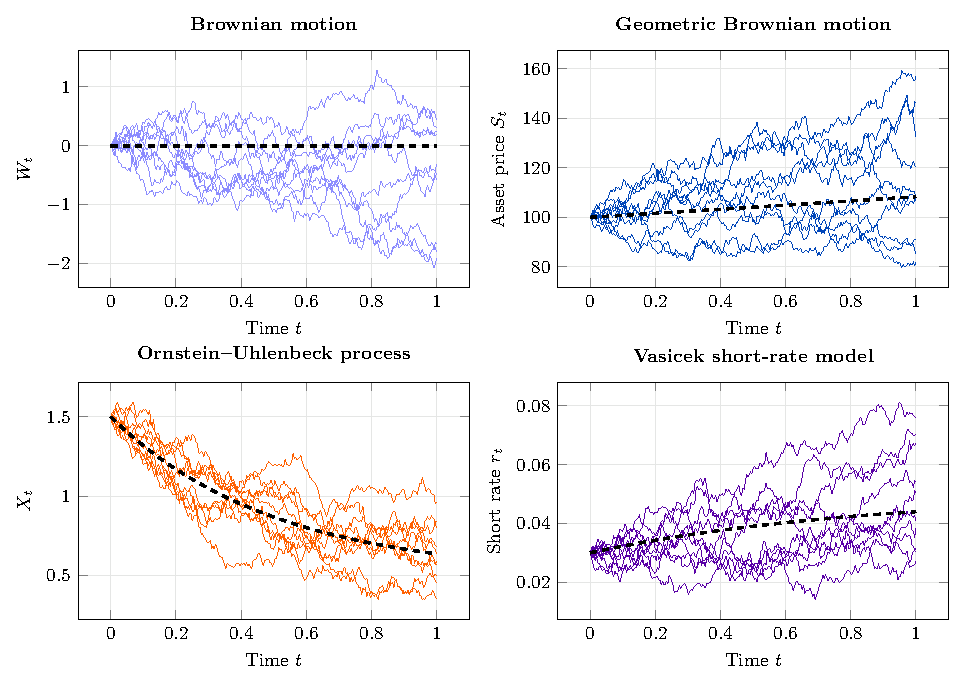
\includegraphics[width=\textwidth]{figures/paths.pdf}
  \caption{Simulated sample paths. Each panel uses ten paths and an exact transition over 252 steps. The dashed line shows the theoretical mean.}
  \label{fig:paths}
\end{figure}

Brownian motion fluctuates around zero and its dispersion increases with time. GBM paths remain positive and fan out asymmetrically because shocks act proportionally to the current price. In the OU panel, all paths begin above $\theta=0.5$ and move downward toward the long-run level. Vasicek paths similarly move from the initial $3\%$ rate toward the $5\%$ long-run level, while random shocks create variation around the expected trajectory.

The distinction between OU and Vasicek is therefore interpretive rather than mathematical: the OU panel represents a generic mean-reverting state variable, whereas the Vasicek panel represents a short interest rate with parameters expressed in rate units.

\subsection{Terminal distributions}

Figure~\ref{fig:distributions} compares histograms from $10{,}000$ simulated terminal values with analytical probability densities. The agreement in shape and location is close for all four models.

\begin{figure}[htbp]
  \centering
  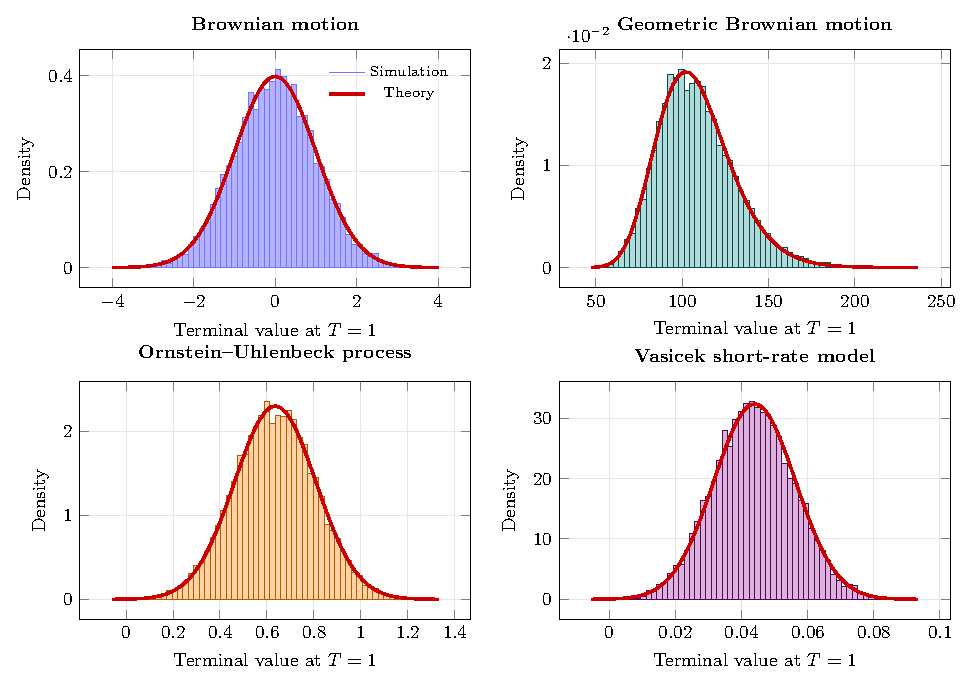
\includegraphics[width=\textwidth]{figures/distributions.pdf}
  \caption{Empirical terminal densities at $T=1$ from $10{,}000$ simulations compared with theoretical densities. Brownian motion, OU, and Vasicek are Gaussian at a fixed time; GBM is lognormal.}
  \label{fig:distributions}
\end{figure}

Brownian motion has a symmetric $\Normal(0,1)$ terminal distribution. GBM has the expected right-skewed lognormal shape. OU and Vasicek have Gaussian terminal distributions, but their centres and variances differ because of their parameter choices. The Vasicek density is concentrated around a rate slightly below its $5\%$ long-run mean because the one-year horizon is not long enough for complete mean reversion from $r_0=3\%$.

\subsection{Moment consistency check}

Table~\ref{tab:diagnostics} compares empirical moments from the $10{,}000$ terminal values with exact theoretical moments. Small differences are expected because Monte Carlo estimates have sampling error.

\begin{table}[htbp]
\centering
\caption{Empirical and theoretical terminal moments at $T=1$.}
\label{tab:diagnostics}
\small
\begin{tabular}{lrrrr}
\toprule
Model & Empirical mean & Theoretical mean & Empirical variance & Theoretical variance\\
\midrule
Brownian motion & $-0.00554$ & $0.00000$ & $0.99262$ & $1.00000$\\
GBM & $108.66319$ & $108.32871$ & $494.96298$ & $478.91887$\\
OU & $0.63246$ & $0.63534$ & $0.03010$ & $0.03006$\\
Vasicek & $0.04368$ & $0.04398$ & $0.0001513$ & $0.0001515$\\
\bottomrule
\end{tabular}
\end{table}

The Brownian empirical variance differs from its target by less than one percent. GBM has the largest variance discrepancy, approximately $3.4\%$, because its right-skewed distribution makes the sample variance more sensitive to unusually high terminal prices. The OU and Vasicek empirical moments are both close to theory. These results, together with the density overlays, provide a numerical consistency check for the exact-transition implementation.

\section{Comparison of the Models}

\begin{table}[htbp]
\centering
\caption{Conceptual comparison of the four processes.}
\label{tab:comparison}
\begin{tabular}{p{2.6cm}p{2.4cm}p{2.4cm}p{3.0cm}p{3.0cm}}
\toprule
Model & State space & Terminal law & Main feature & Typical limitation\\
\midrule
Brownian motion & $\mathbb{R}$ & Normal & Independent additive increments & Can be negative; not a direct stock-price model\\
GBM & $(0,\infty)$ & Lognormal & Proportional shocks and positivity & Constant volatility; no jumps or mean reversion\\
OU & $\mathbb{R}$ & Normal & Mean reversion & Can be negative; constant absolute volatility\\
Vasicek & $\mathbb{R}$ & Normal & Mean-reverting short rate and affine bond prices & Allows unrestricted negative rates\\
\bottomrule
\end{tabular}
\end{table}

No single process is universally best. The model should reflect the economic variable and the features relevant to the application. Brownian motion is the fundamental noise process. GBM is suitable when changes are naturally proportional to a positive level. OU is suitable when deviations from an equilibrium tend to decay. Vasicek retains OU tractability while giving its parameters a term-structure interpretation.

All results here use constant parameters and one stochastic factor. Real markets may require time-varying parameters, correlated factors, jumps, stochastic volatility, regime changes, or calibration to observed data. Simulated paths demonstrate implications of assumptions; they do not establish that those assumptions describe a particular market.

\section{Conclusion}

The simulations reproduce the principal theoretical features of four important stochastic processes. Brownian motion exhibits independent Gaussian increments with variance increasing linearly in time. GBM transforms Brownian shocks into positive, lognormally distributed asset prices. The OU process introduces an explicit pull toward a long-run mean. The Vasicek model applies the same Gaussian mean-reverting mechanism to short-term interest rates and provides analytical bond prices.

Exact transition equations make the simulation both simple and free of Euler discretisation bias at the grid points. The empirical terminal densities and moments agree closely with their analytical counterparts, providing a numerical consistency check. At the same time, the comparison highlights that tractability comes with restrictive assumptions. Understanding both the mathematical behaviour and the financial limitations of each process is necessary before applying it to pricing, risk management, or forecasting.

\appendix
\section{Reproducibility}

The project is implemented in Python using only the standard library, with \texttt{uv} managing the Python environment. Fixed-seed output is exactly reproducible when the same Python version is used. The figures are rendered as vector graphics with LaTeX and PGFPlots. From the project directory, the complete results can be regenerated using:
\begin{verbatim}
uv run python -m unittest -v test_simulation.py
uv run python generate_data.py
latexmk -pdf -output-directory=figures figures/paths.tex
latexmk -pdf -output-directory=figures figures/distributions.tex
latexmk -pdf main.tex
\end{verbatim}

The test suite checks Brownian moments, GBM positivity and expected value, deterministic OU mean reversion, equivalence of the OU and Vasicek transitions, fixed-seed reproducibility, and correct histogram bin-edge output. Generated data are stored as CSV files so that every plotted point can be inspected independently of the plotting software.

\begin{thebibliography}{9}

\bibitem{shreve}
S. E. Shreve,
\textit{Stochastic Calculus for Finance II: Continuous-Time Models},
Springer, 2004.

\bibitem{glasserman}
P. Glasserman,
\textit{Monte Carlo Methods in Financial Engineering},
Springer, 2004.

\bibitem{hull}
J. C. Hull,
\textit{Options, Futures, and Other Derivatives}, 11th ed.,
Pearson, 2021.

\bibitem{vasicek}
O. Vasicek,
``An Equilibrium Characterization of the Term Structure,''
\textit{Journal of Financial Economics}, vol. 5, no. 2, pp. 177--188, 1977.

\bibitem{ou}
G. E. Uhlenbeck and L. S. Ornstein,
``On the Theory of the Brownian Motion,''
\textit{Physical Review}, vol. 36, pp. 823--841, 1930.

\end{thebibliography}

\end{document}
